%!TEX root = thesis.tex

\appendix


% -------------------------------------------------------------
\chapter{Field Study Survey}
\label{appendix:field-study-survey}

This survey was presented to the audience through an option of either a paper-based or online medium.

\clearpage

\begin{center}
\fbox{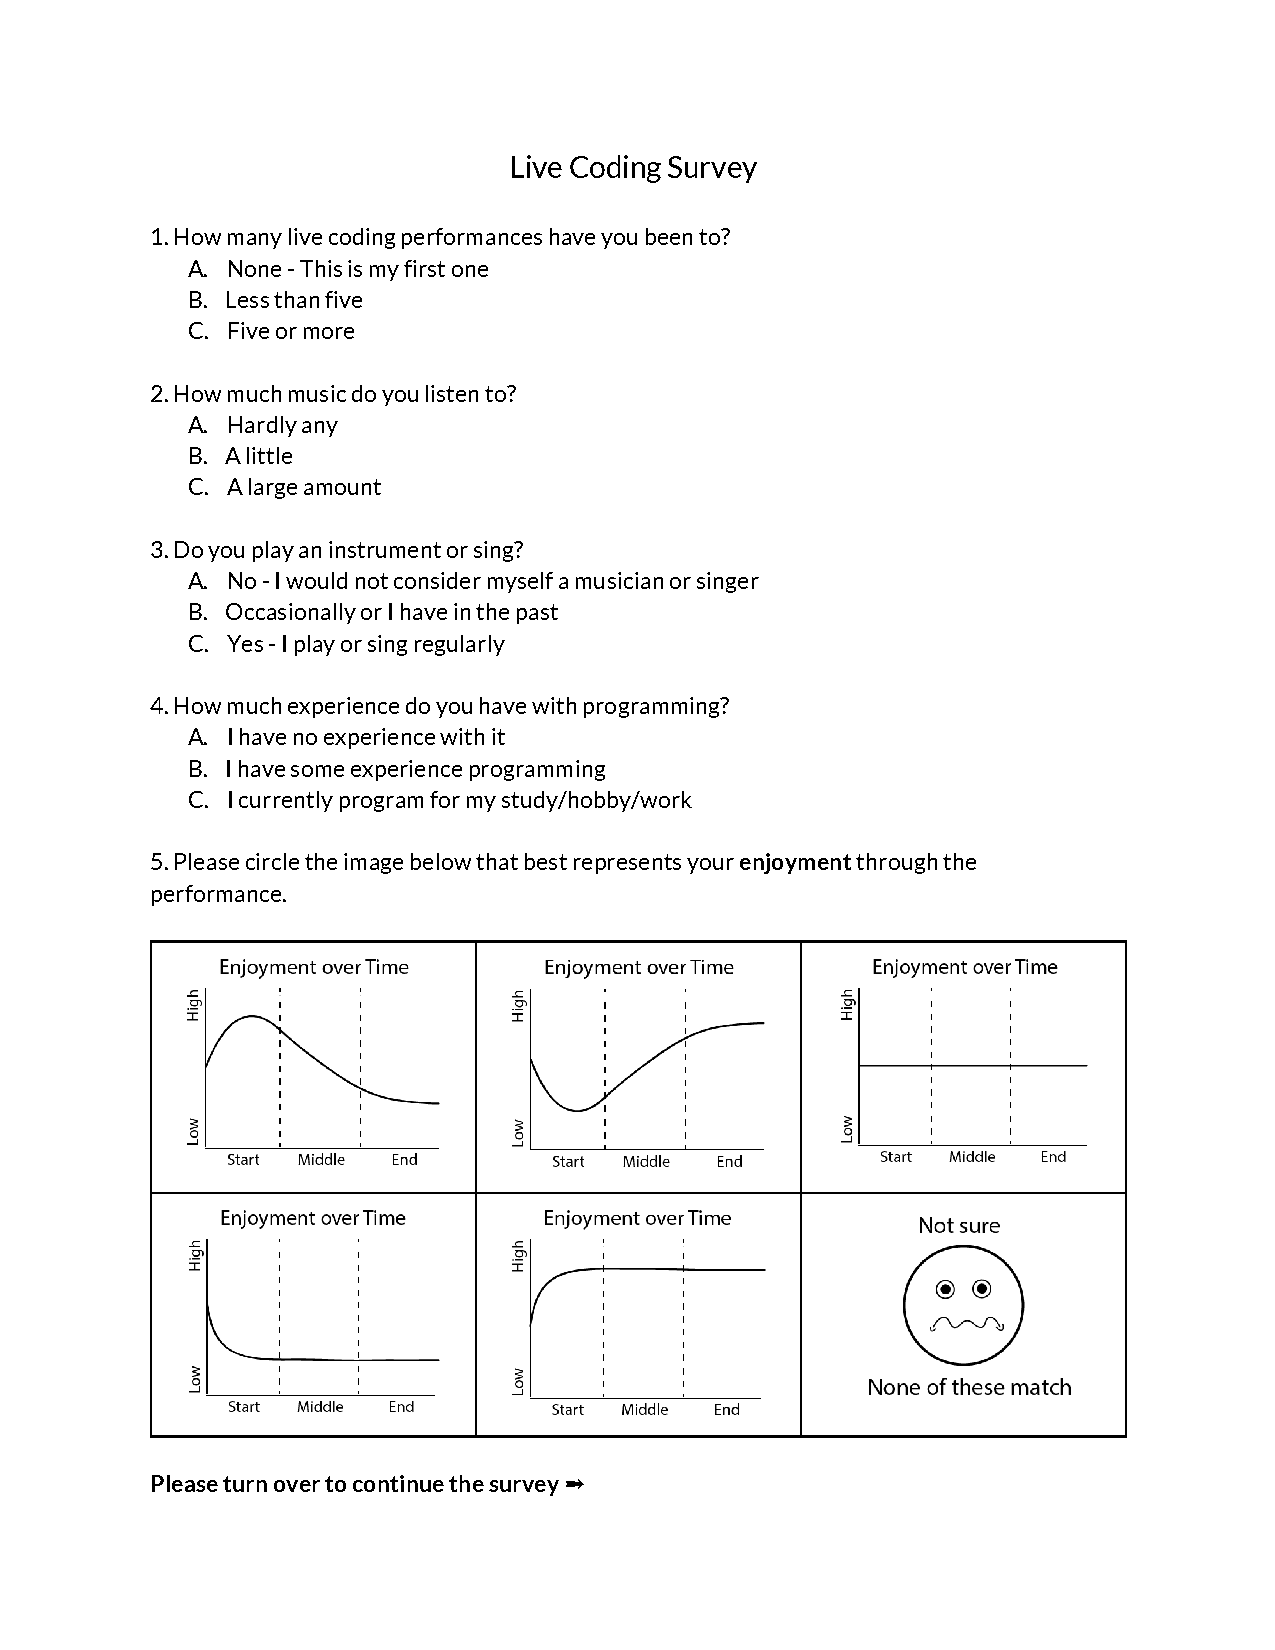
\includegraphics[page=1,width=\textwidth]{../study-1/survey/live-coding-survey-final.pdf}}
\end{center}

\begin{center}
\fbox{\includegraphics[page=2,width=\textwidth]{../study-1/survey/live-coding-survey-final.pdf}}
\end{center}

\chapter{Field Study Survey Results}
\label{appendix:field-study-survey-results}

A summary of the initial exploratory field study survey results are presented below. These results were gathered from the survey presented above.


% -------------------------------------------------------------
\chapter{Field Study Follow-Up Interviews}
\label{appendix:field-study-follow-up-interviews}

The initial exploratory field study prompted a number of questions. These questions were developed further through a number of email based follow-up interviews. A summary of the results are presented below.


\section*{Interviewee 1}
\textit{Question 1: What did you ``understand'' about what was going on with the code being projected? In particular, what did you understand about the relationship between the code and the music?}

The code sets up a set of nested loops which are then modified by the composer in real time. This immediately leads to the danger of repetitive loops. It may be useful to have rhythms of 4 or 8 bar repetition as in Africa. Actually, this musical form lends itself to that type of rhythm and music. As soon as an organ comes in I am reminded of Mike Oldfield and am anxious that someone will say “slightly distorted guitar”. In jazz one improvises on standards so there is a very strong form (AABA etc) which, in general, is respected allowing the audience to deduce where they are in the piece. I had the feeling that the present way the code is used limited the music

\textit{Question 2: Would would you like to understand more about the code in order to enjoy the performance more?}

Yes, I think that if the audience were told what was happening or the ideas behind the constructs then I would be happier. Compared to jazz it is not note by note improvisation so an explanation of the limits and advantages would be useful.

\section*{Interviewee 2}

\textit{Question 1: What did you ``understand'' about what was going on with the code being projected? In particular, what did you understand about the relationship between the code and the music?}

In the beginning, I could tell from the silence and the live coding that it was being build, and sound by sound line by line was being added to as the piece grew.  When [the live coder] went back in the code to change beats or melodies, I could tell something was being changed but wasn't tracking what or how.

\textit{Question 2: Would would you like to understand more about the code in order to enjoy the performance more?}

I feel like I already understood a rudimentary amount [...] which was enough to enjoy it.  I feel like if I had more knowledge about code I would focus on that to the detriment of the music; and if I knew more about music then I may have focused on that to the detriment of my attention on the code.  Considering my education, if I had not had the exposure to code and music through [...], then some basic rudimentary knowledge of code would have been good.

\section*{Interviewee 3}

\textit{Question 1: What did you ``understand'' about what was going on with the code being projected? In particular, what did you understand about the relationship between the code and the music?}

I understood that the music was being made from scratch and this was evident in the long silence before any sound is heard. I understand what sounds are being made based on the code names and that some of the numbers represent timing, volume and pitch.  I still don't quite understand when the code is ``ready'' and starts working to make music. It has something to do with the highlighting the text, but that also confuses me. (I understand that most of the music is stored in the program as ``sound bites'' of real instruments, but sounds can also be made from scratch as mathematical wave functions [...]). Sometimes the coder scrolls up and down the screen to much and I get lost, I don't have a big picture of what all the code looks like.

\textit{Question 2: Would you like to understand more about the code in order to enjoy the performance more?}

In some ways I would like to understand a little more about the code. It would be nice to have a director's commentary of what's going on behind the scenes, just so I can follow along with the changes that I can hear in the music as they are occurring. But I think I more enjoy just listening to the music, knowing broadly that a livecoder is manipulating code to make the sounds that I hear. I don't often like reading the code for the whole performance, maybe for a few minutes at a time, but then I like to switch off and just focus on what the musician is playing. I more often like to listen to the music and guess what the livecoder has done to make that changes (which is kind of backwards). I wouldn't mind having more understanding of the code on hand, but I probably wouldn't use the details of it during the whole performance every time.



% -------------------------------------------------------------
\chapter{User Study Visualisations}
\label{appendix:user-study-visualisations}

The initial iteration of eight visualisations developed included two sets of four for the aesthetic condition and the didactic condition. Representative screenshots of the visual animations are presented below.

-list all visualisations here

\section*{Aesthetic Condition}

\section*{Didactic Condition}



% -------------------------------------------------------------
\chapter{User Study Advertisement}
\label{appendix:user-study-advertisement}

The initial user study was advertised throughout the university campus including through social groups and posters. The poster used to advertise the study is included below for reference.

\begin{center}
\fbox{
\includegraphics[page=1,width=\textwidth]{../study-2/documents/live-coding-flyer-30-5-2014.pdf}}
\end{center}

\chapter{User Study Survey}
\label{appendix:user-study-survey}

The initial user study investigated the application of the developed visualisation to the space of live coding computer music performance. The survey used to evaluate these visualisations is presented below.

\clearpage

\begin{center}
\fbox{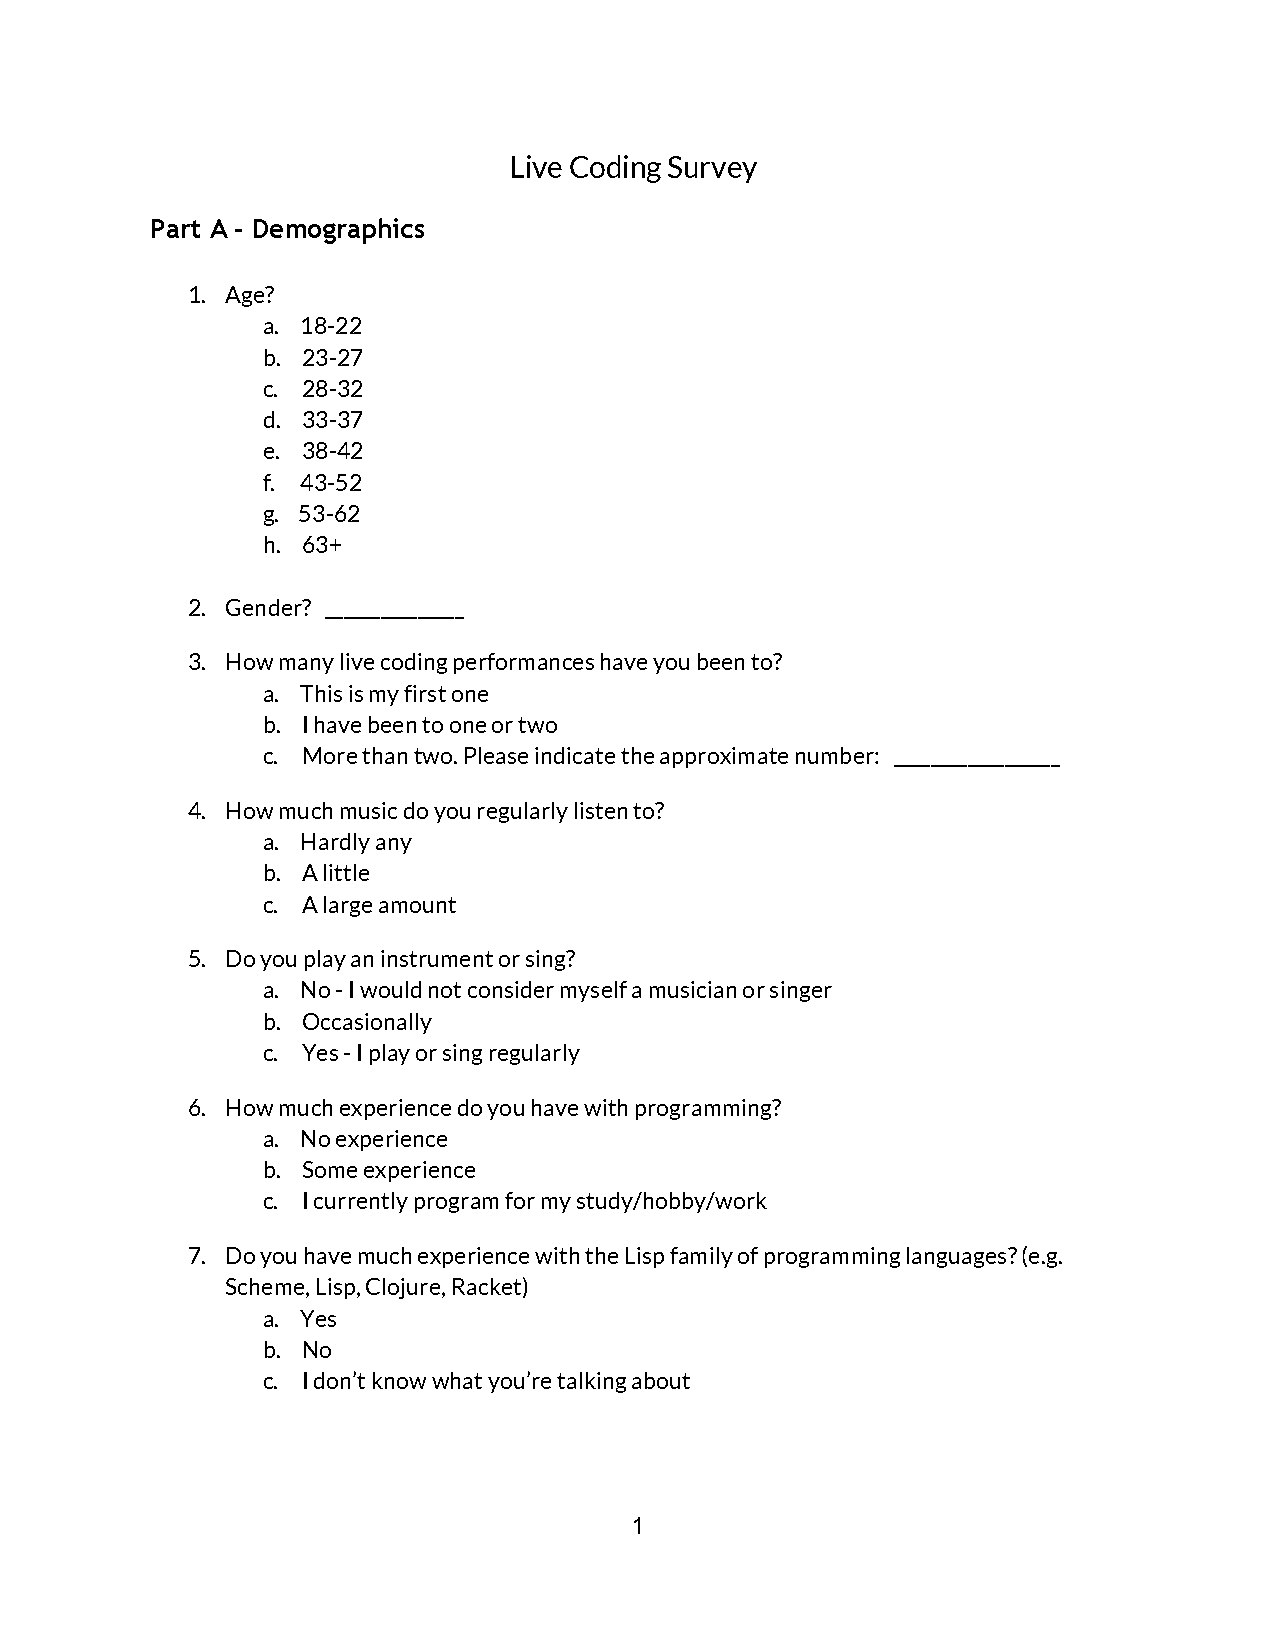
\includegraphics[page=1,width=\textwidth]{../study-2/documents/survey.pdf}}
\end{center}

\begin{center}
\fbox{\includegraphics[page=2,width=\textwidth]{../study-2/documents/survey.pdf}}
\end{center}

\begin{center}
\fbox{\includegraphics[page=3,width=\textwidth]{../study-2/documents/survey.pdf}}
\end{center}

\begin{center}
\fbox{\includegraphics[page=4,width=\textwidth]{../study-2/documents/survey.pdf}}
\end{center}


% -------------------------------------------------------------
\chapter{User Study Survey Results}
\label{appendix:user-study-survey-results}

A summary of the results of the first user study is presented below.

\begin{figure}
    \centering
    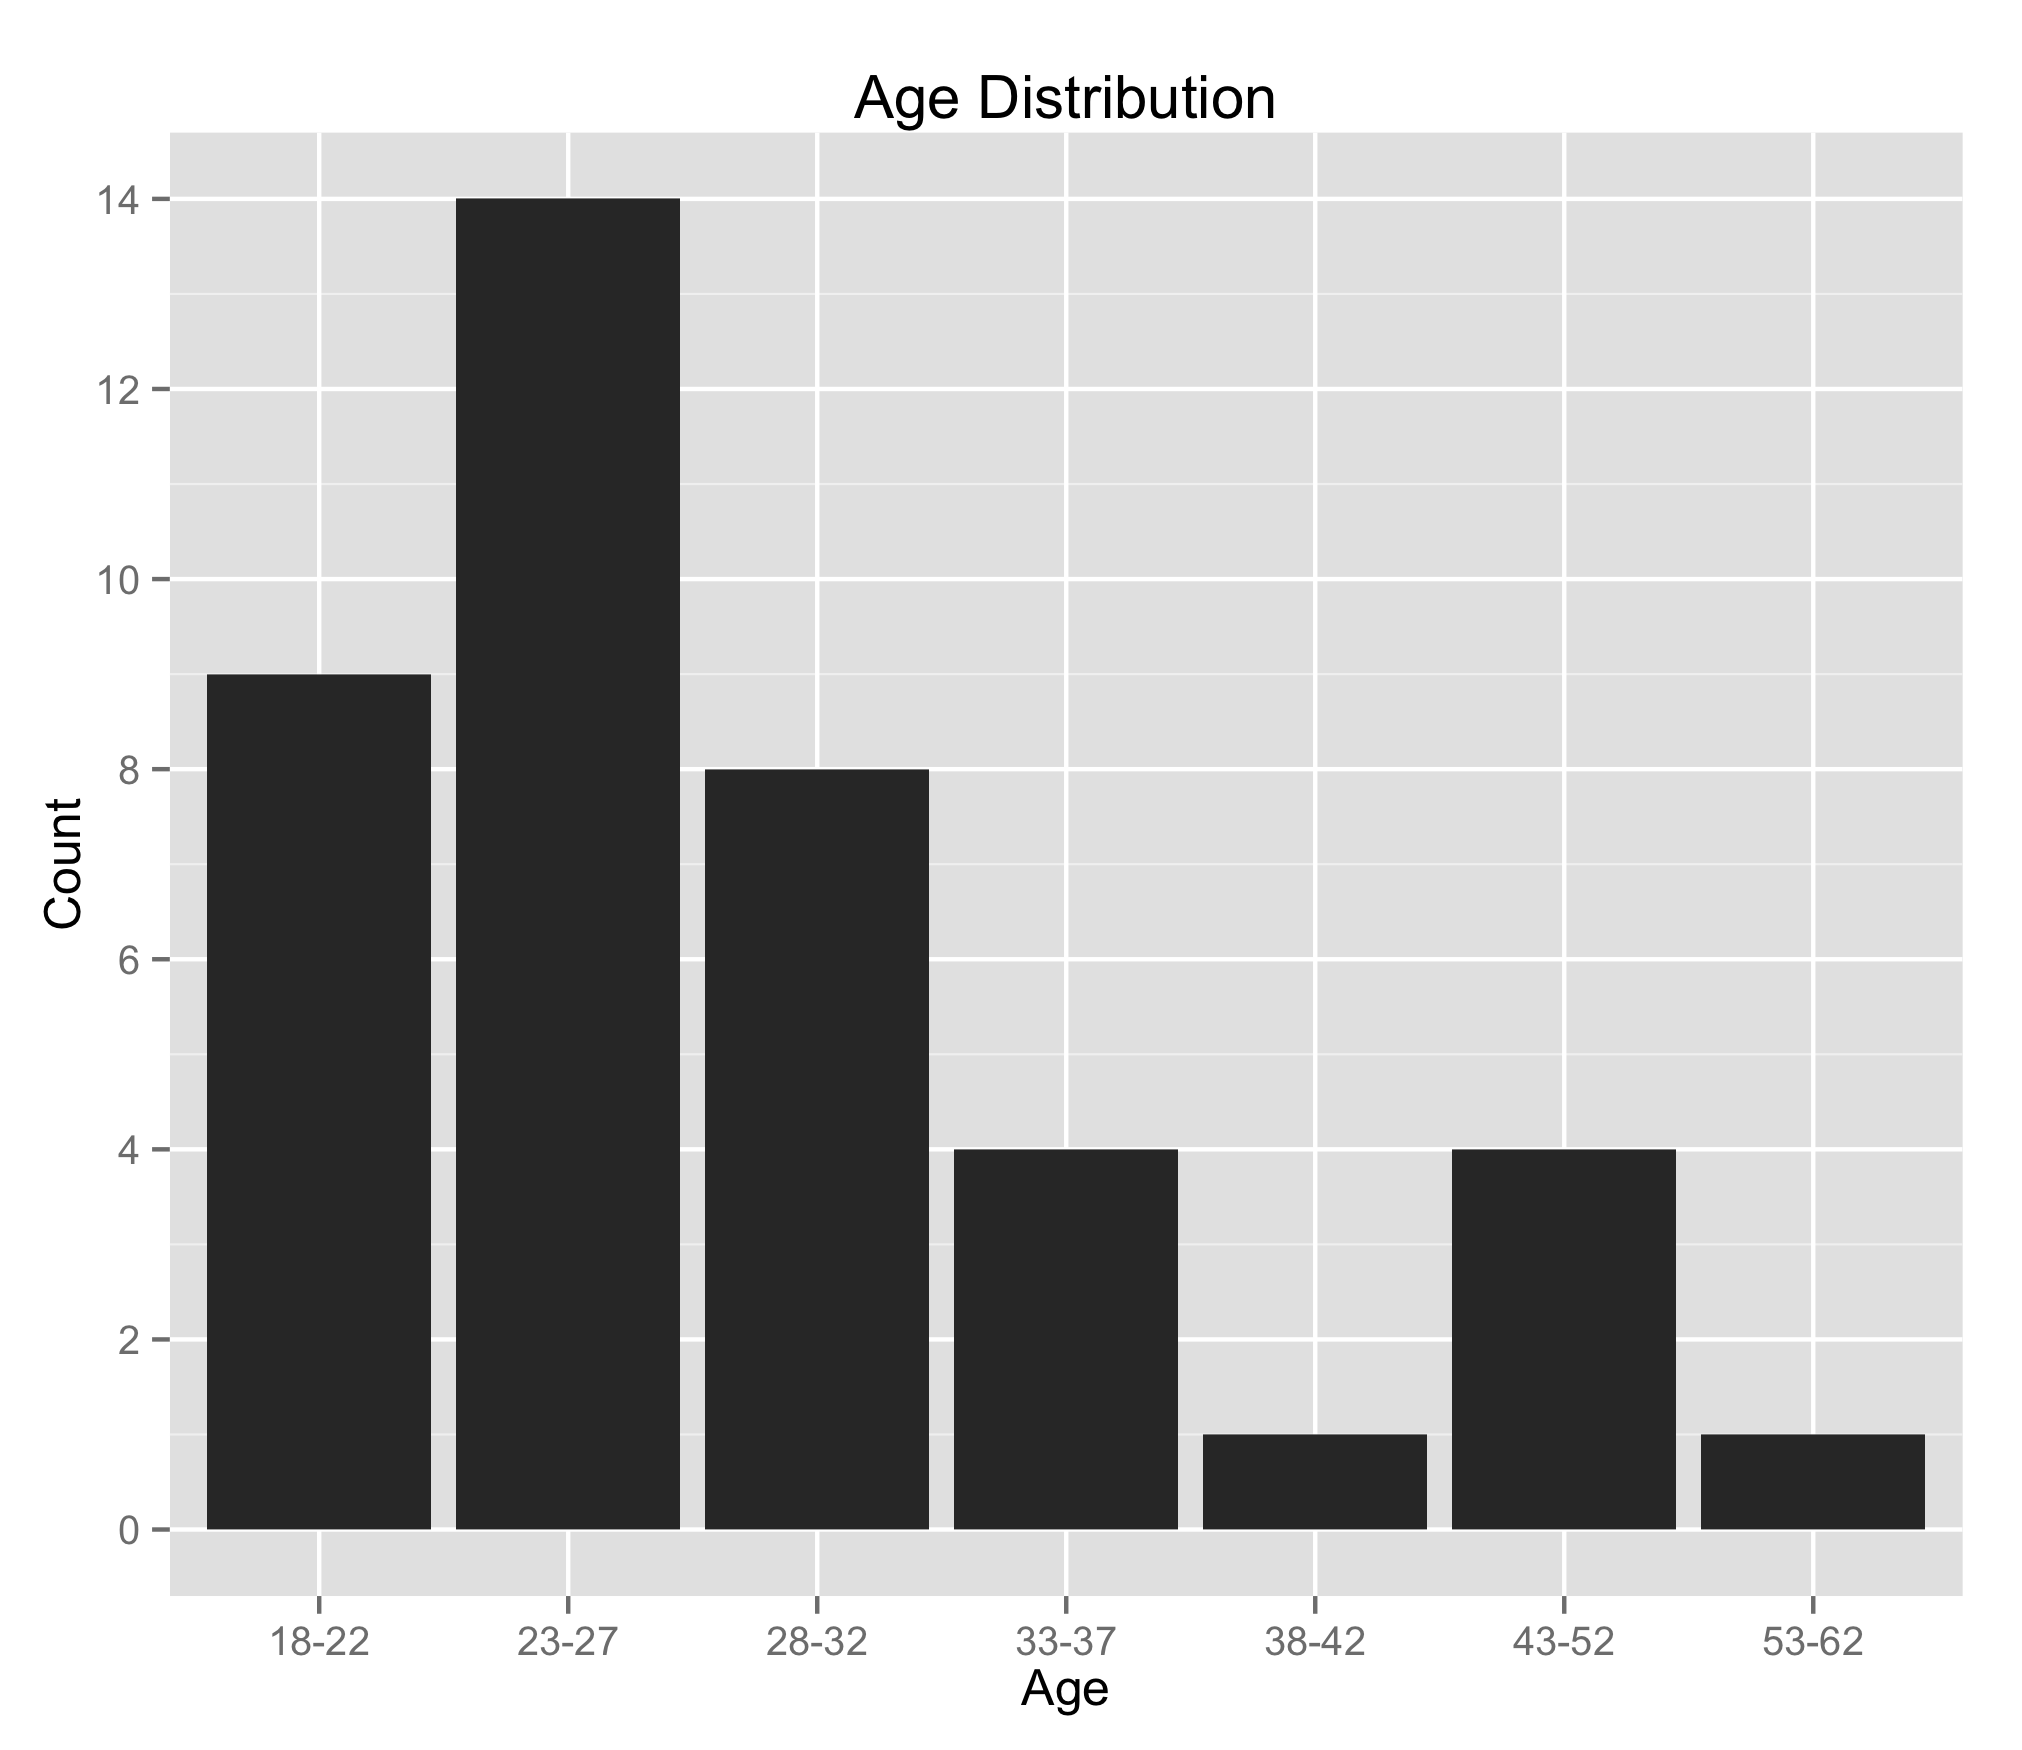
\includegraphics[width=1.0\linewidth]{../study-2/results/graphs/age.png}
    \caption{Age Distribution}
    \label{agedistribution}
\end{figure}

\begin{figure}
    \centering
    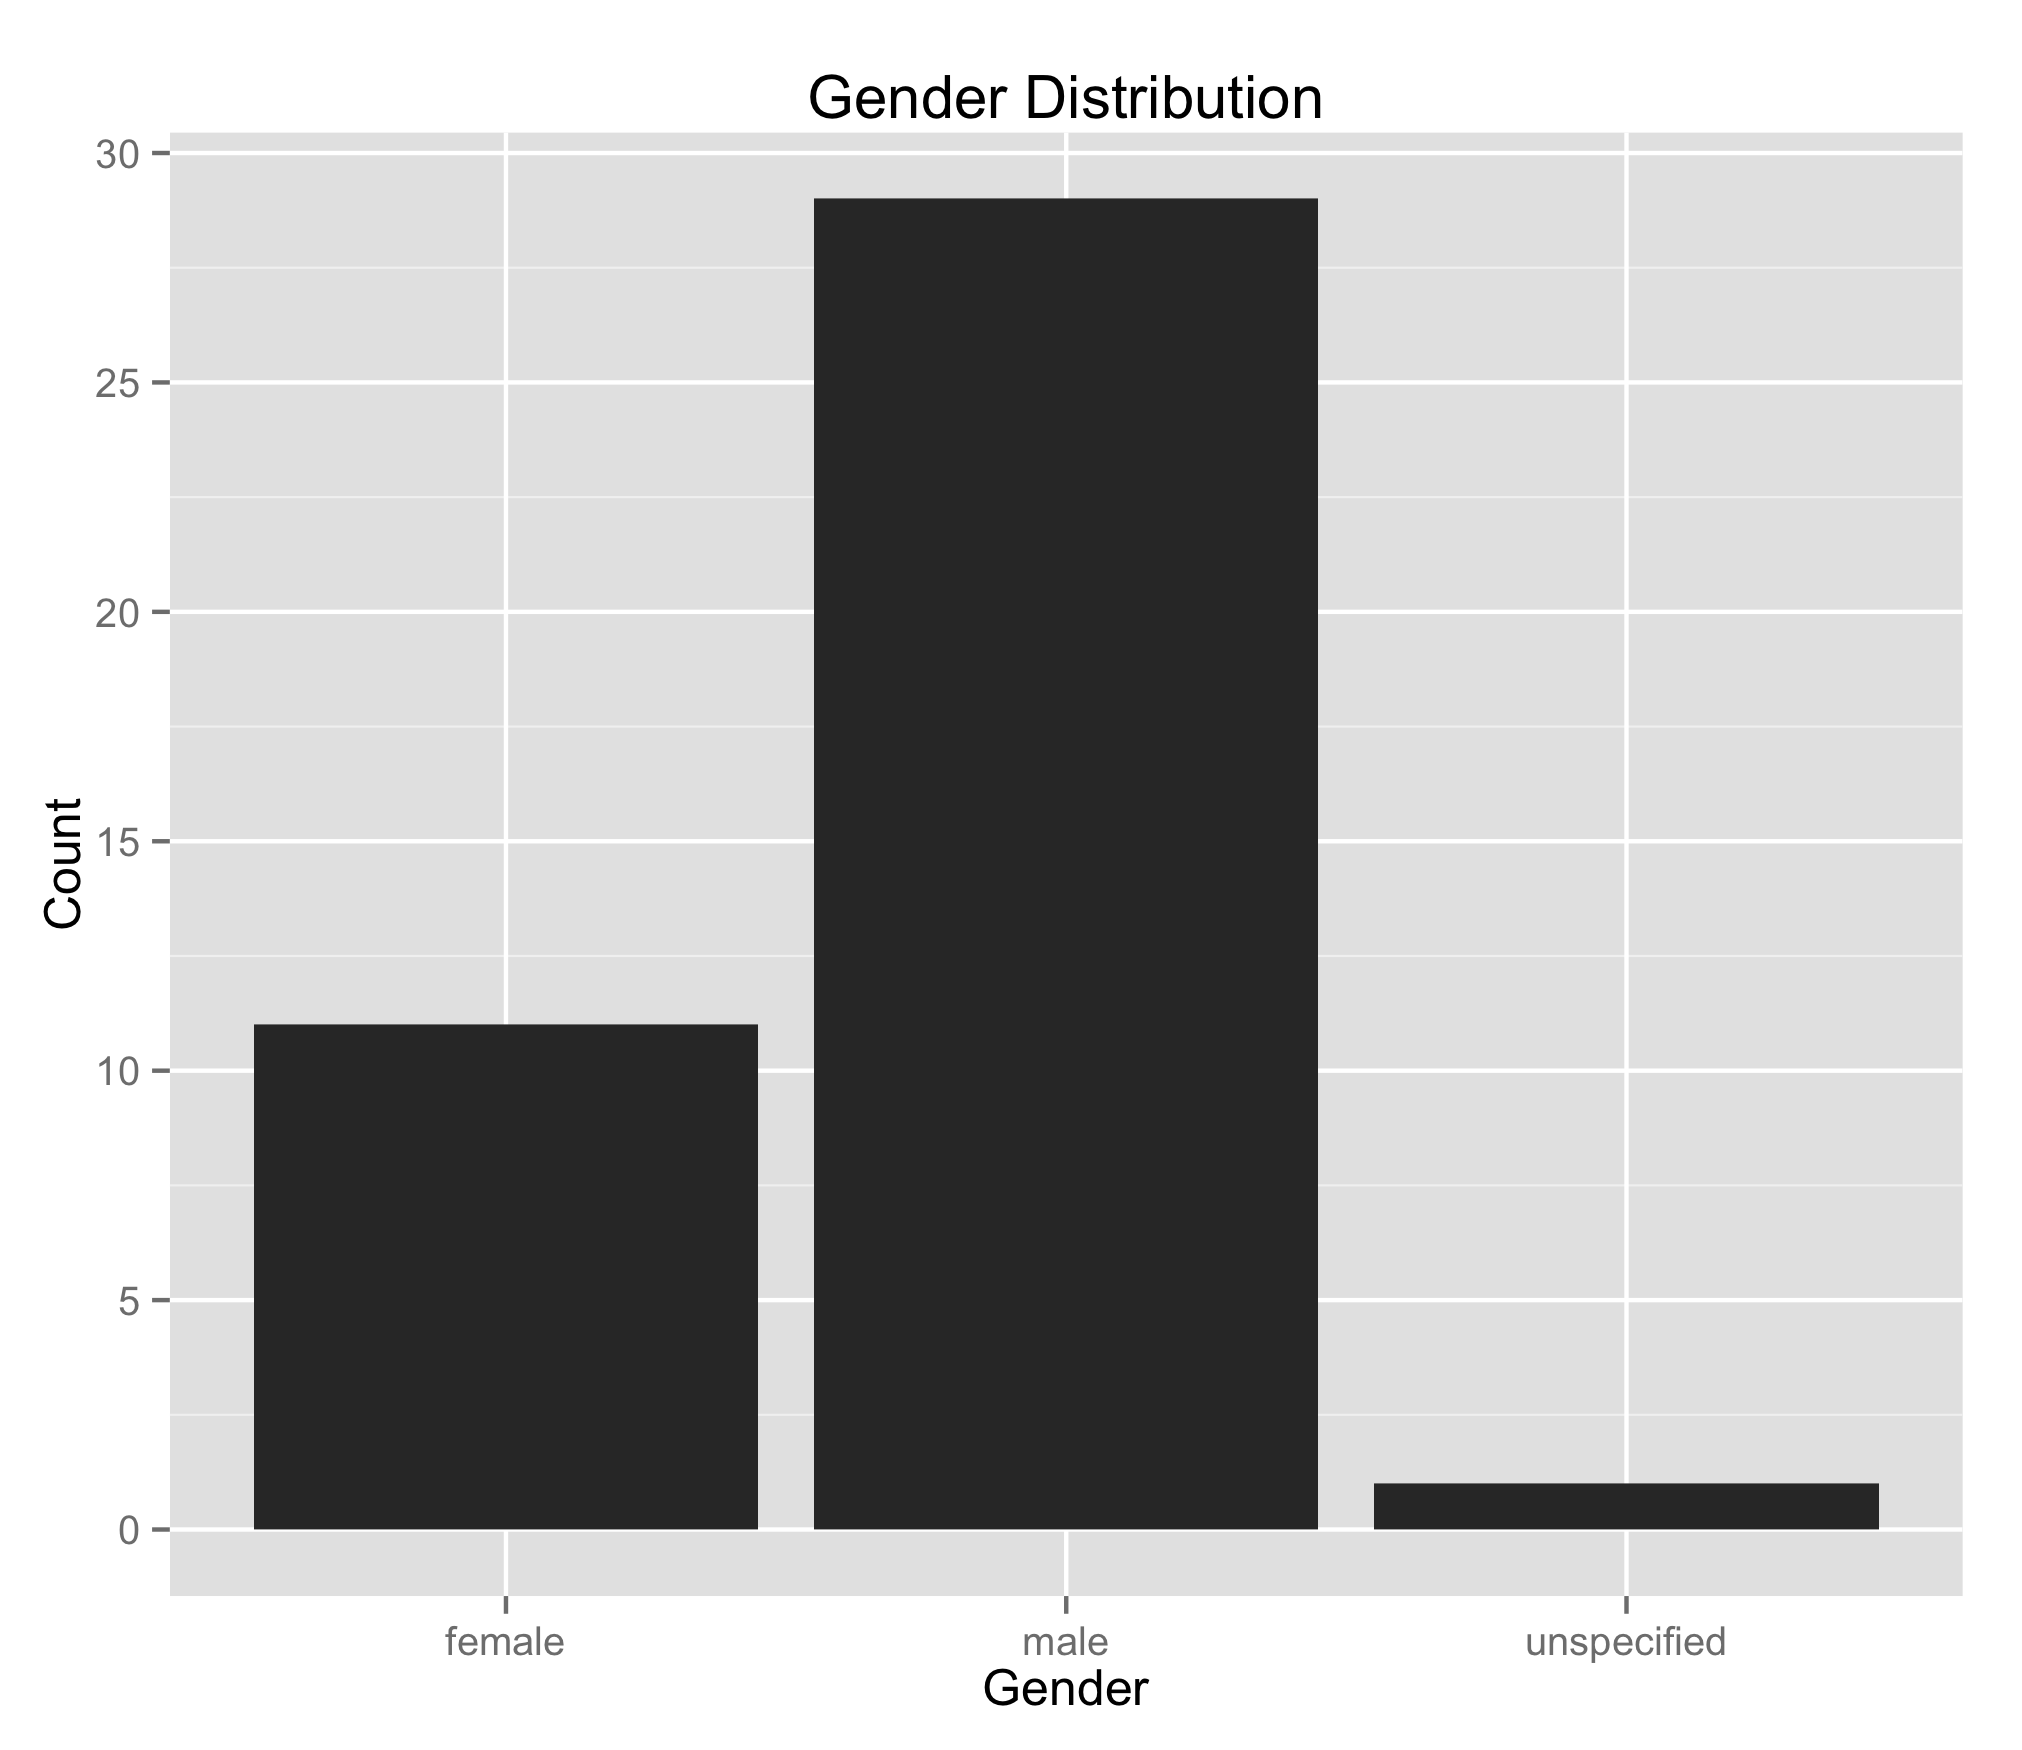
\includegraphics[width=1.0\linewidth]{../study-2/results/graphs/gender.png}
    \caption{Gender Distribution}
    \label{genderdistribution}
\end{figure}

\begin{figure}
    \centering
    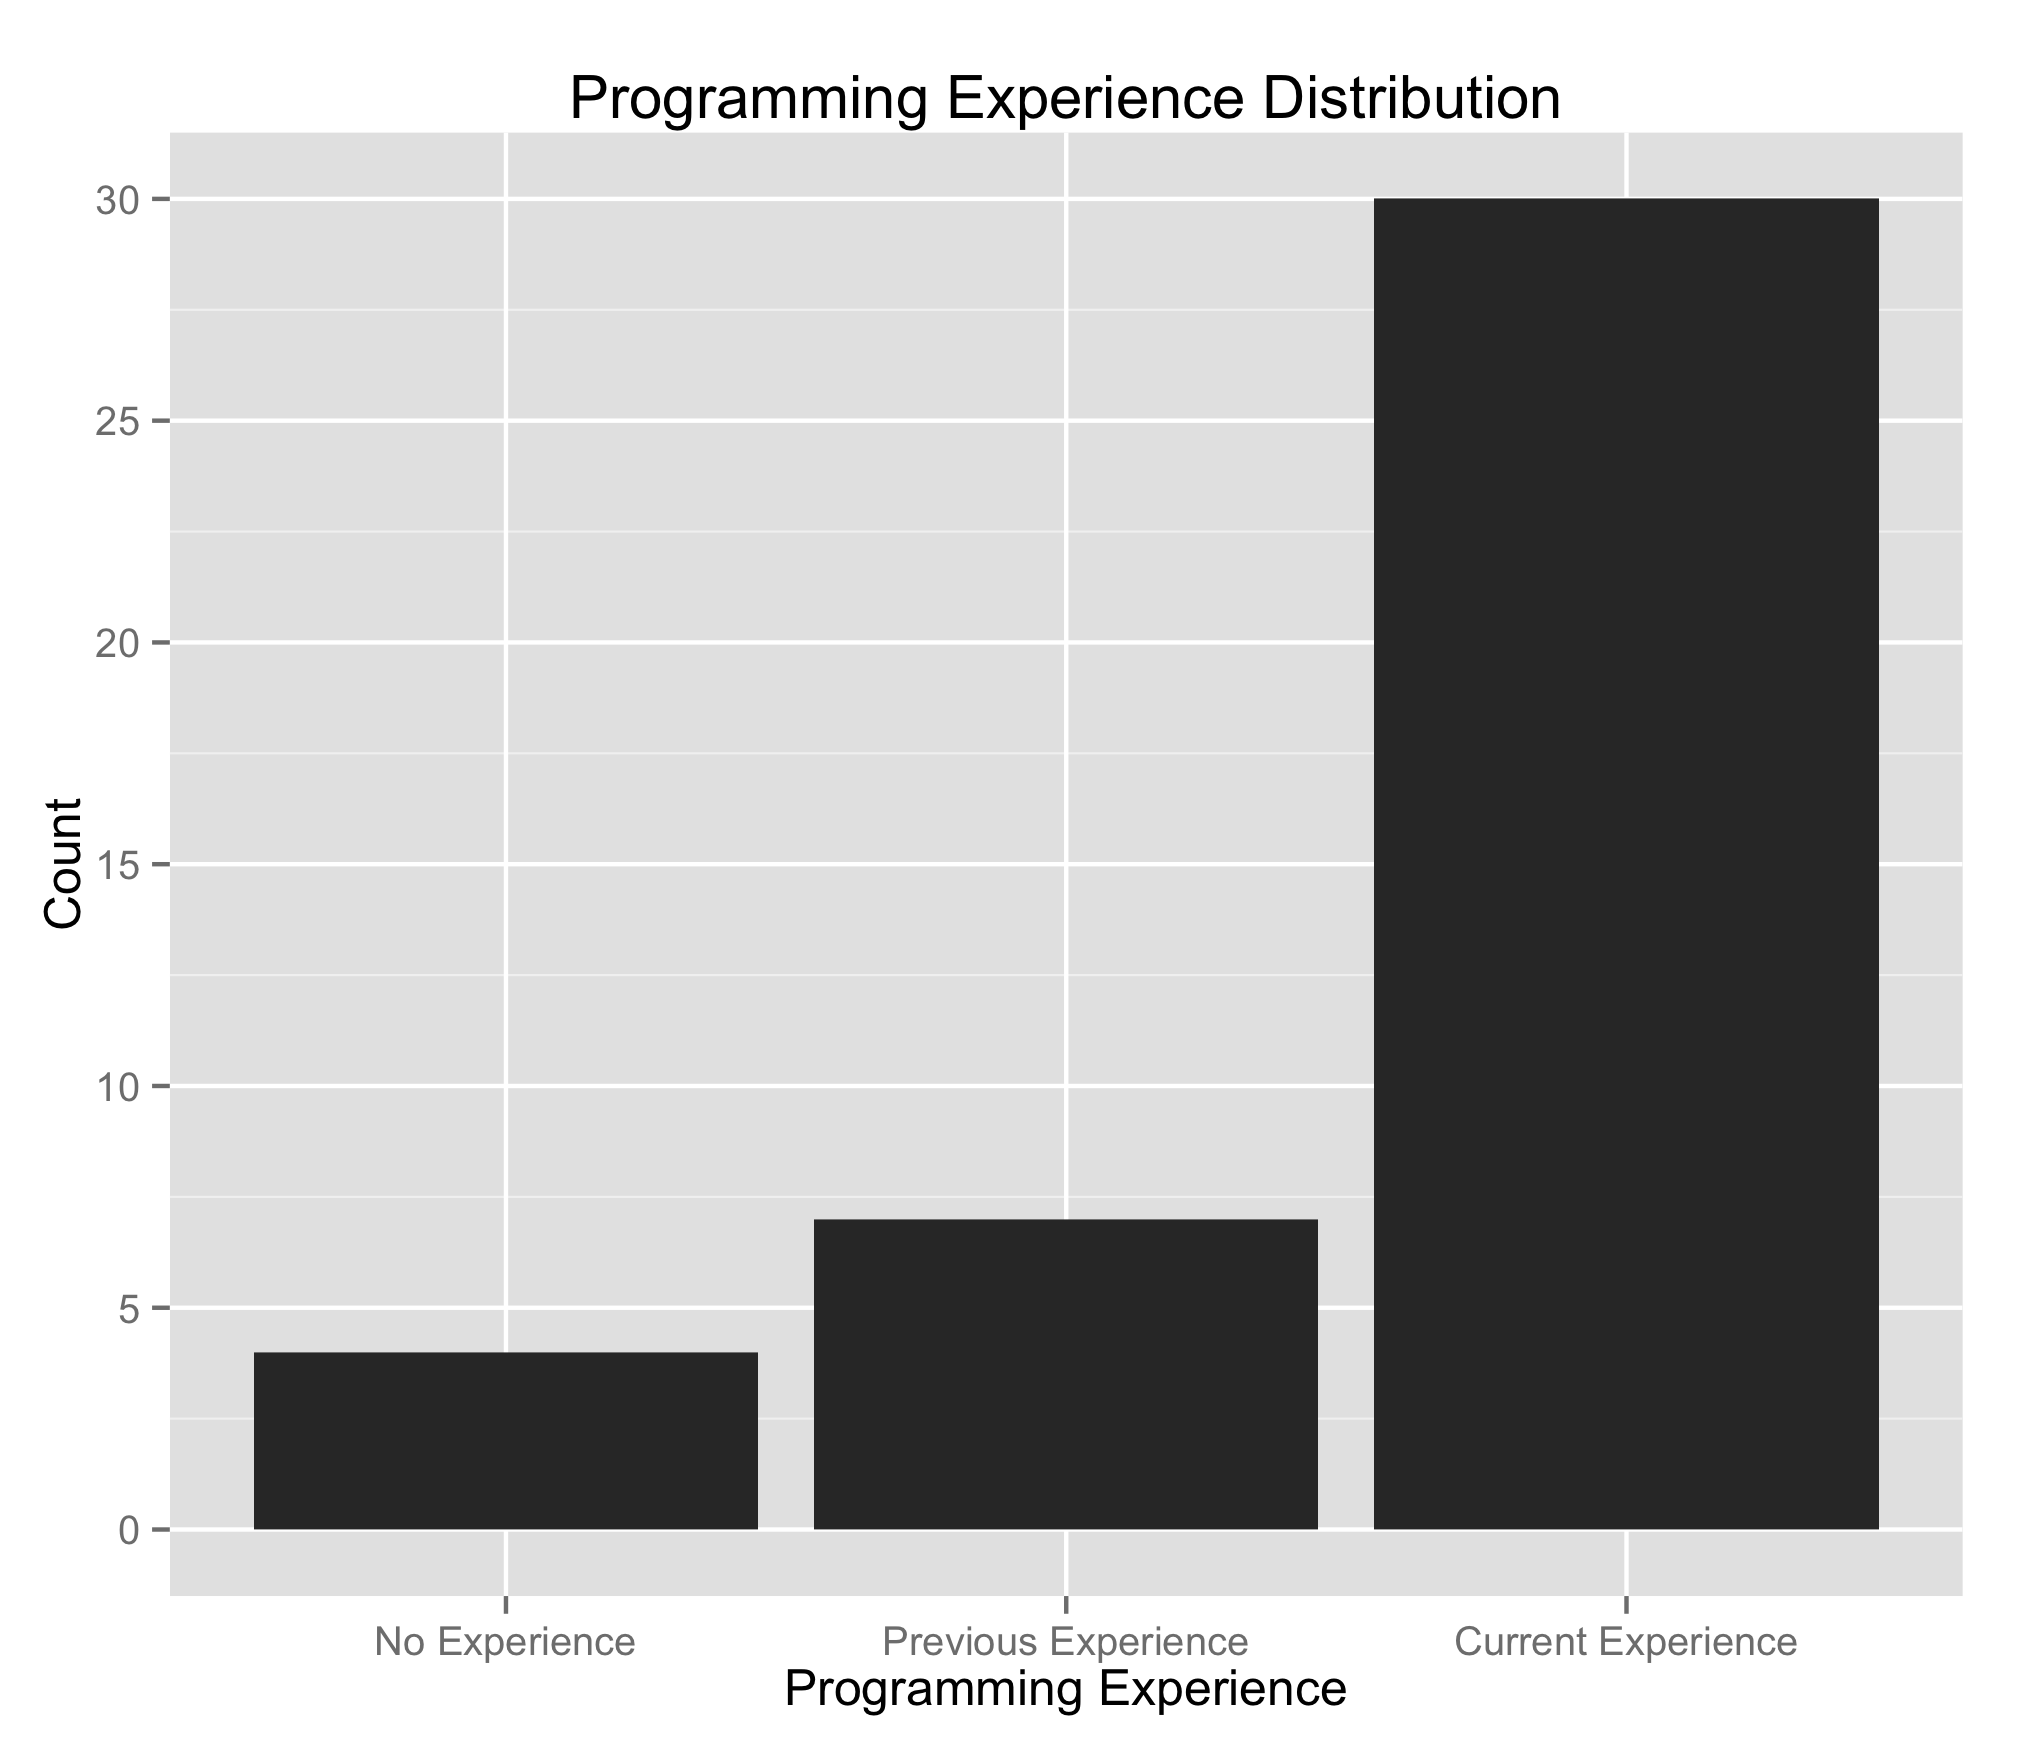
\includegraphics[width=1.0\linewidth]{../study-2/results/graphs/programming.png}
    \caption{Programming Experience Distribution}
    \label{programmingdistribution}
\end{figure}

\begin{figure}
    \centering
    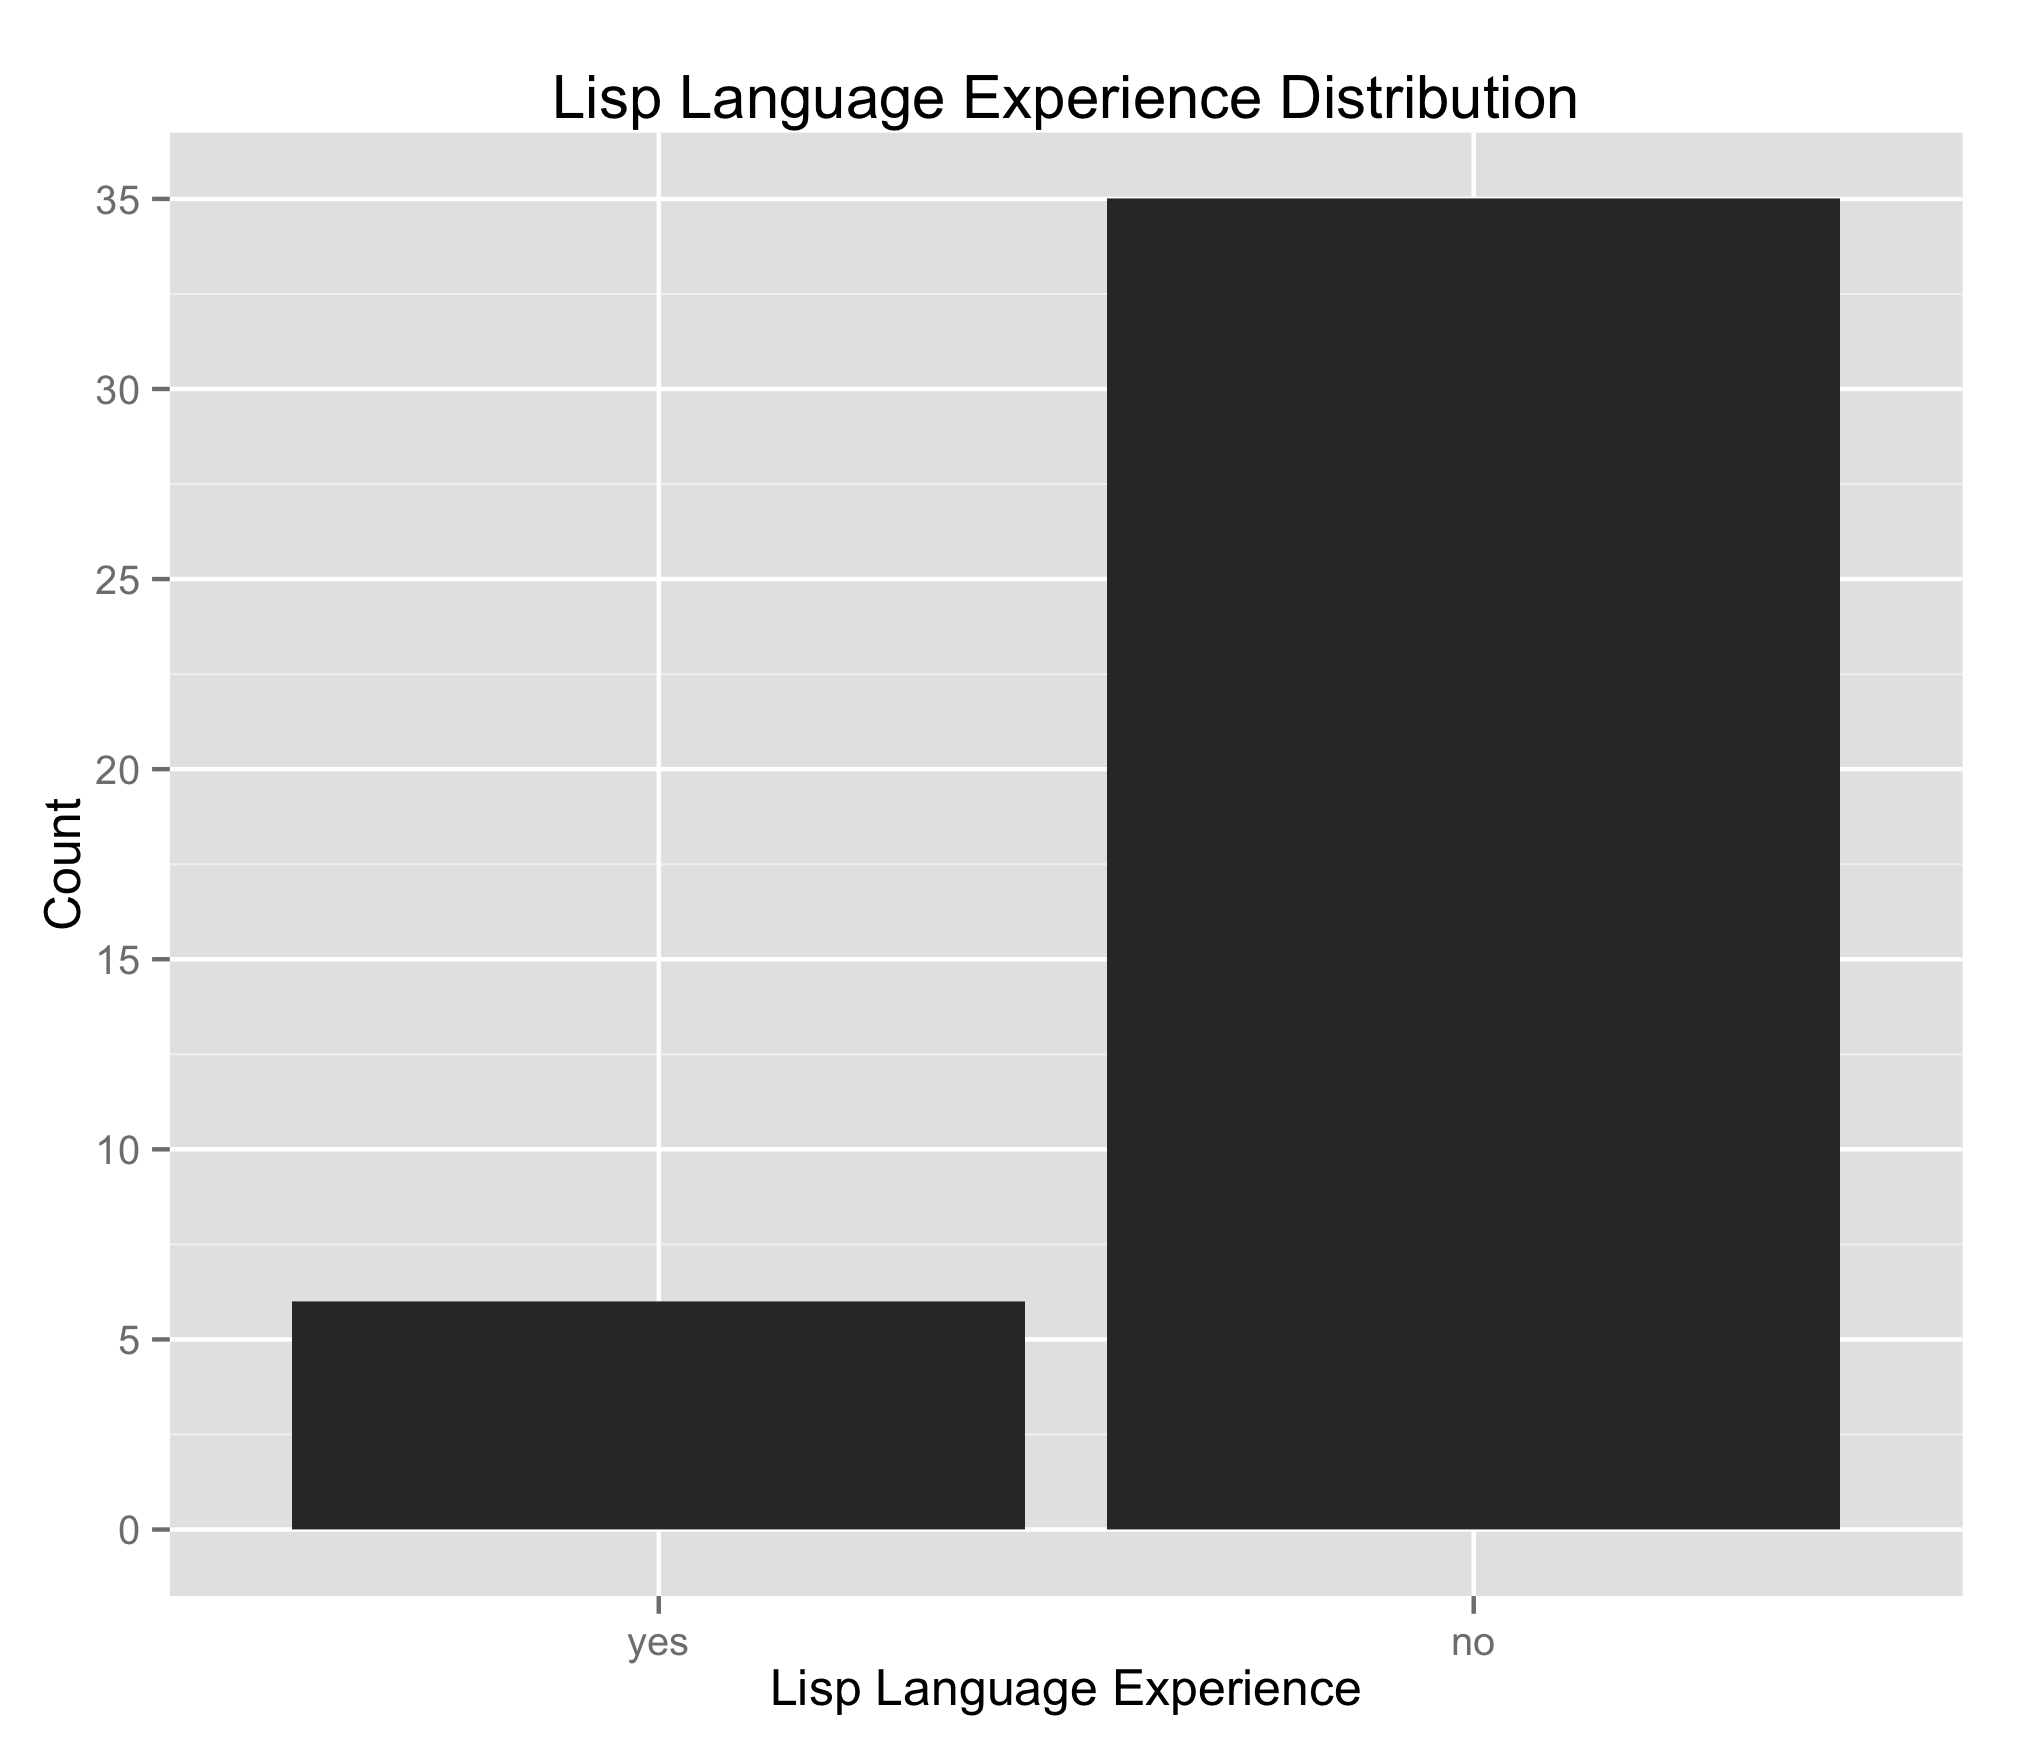
\includegraphics[width=1.0\linewidth]{../study-2/results/graphs/lisp.png}
    \caption{Lisp Experience Distribution}
    \label{lispdistribution}
\end{figure}

\begin{figure}
    \centering
    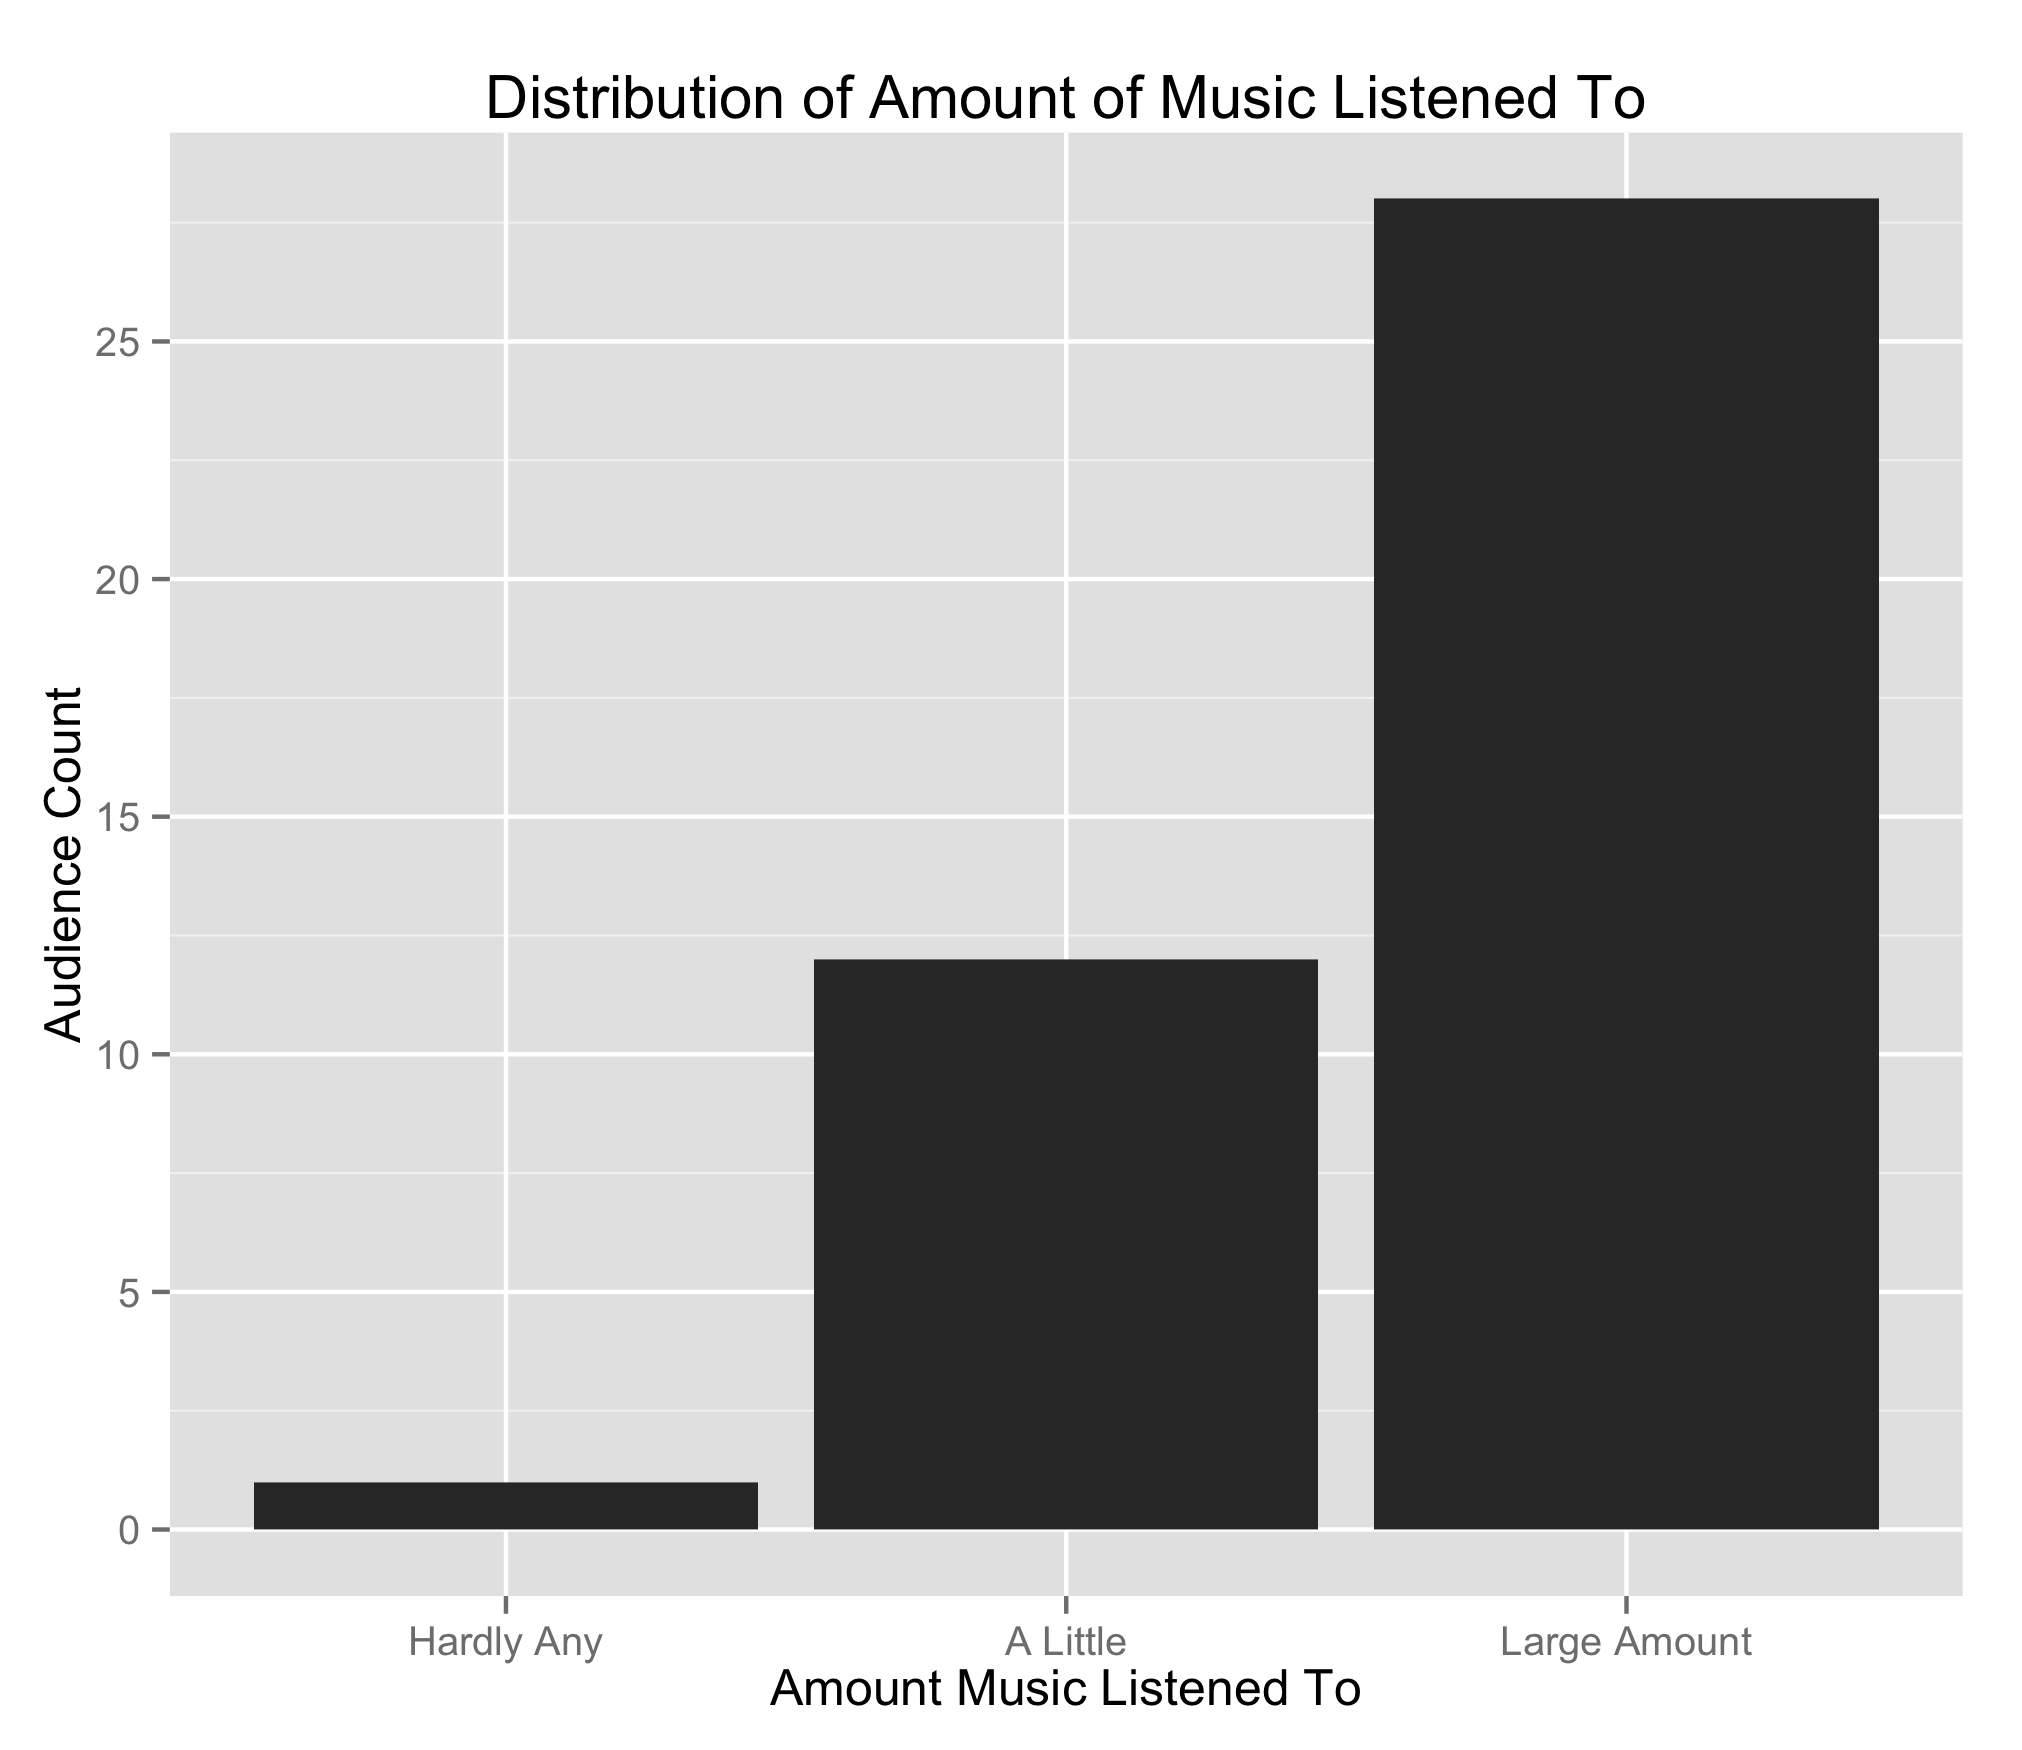
\includegraphics[width=1.0\linewidth]{../study-2/results/graphs/music.png}
    \caption{Listen to Music Regularity Distribution}
    \label{musicdistribution}
\end{figure}

\begin{figure}
    \centering
    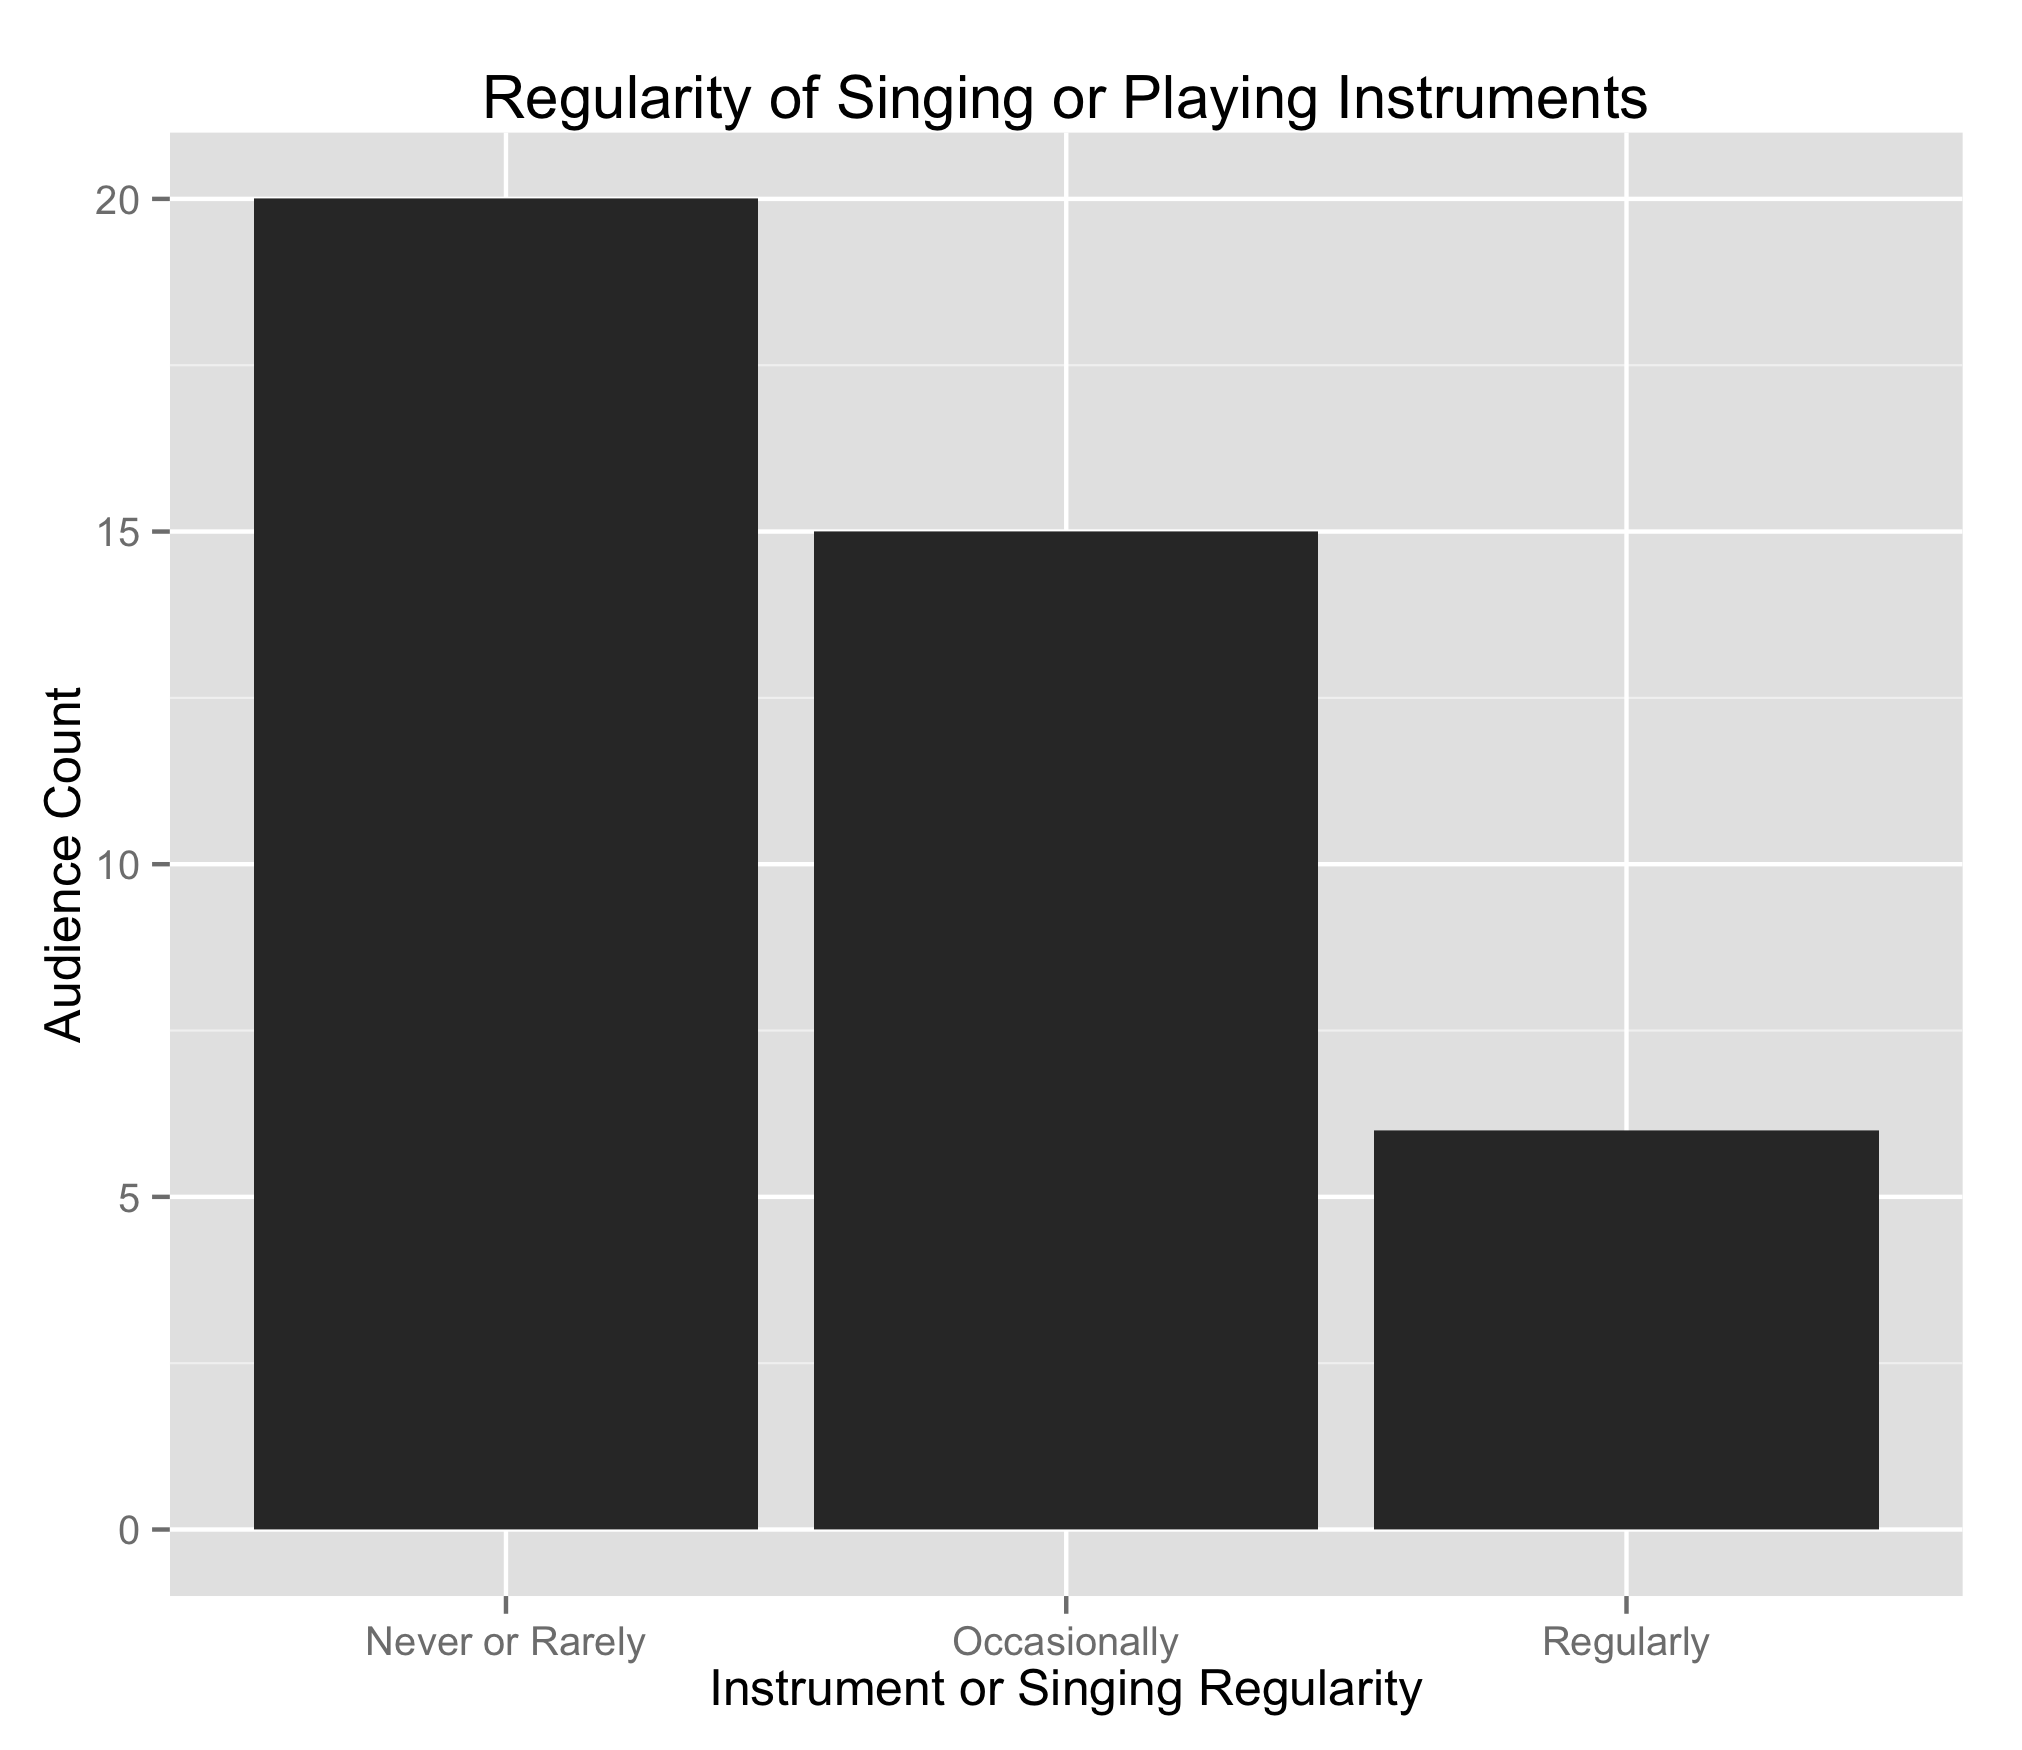
\includegraphics[width=1.0\linewidth]{../study-2/results/graphs/instrument-regularity.png}
    \caption{Playing Instrument or Singing Regularity Distribution}
    \label{instrumentdistribution}
\end{figure}



% -------------------------------------------------------------
\chapter{Live Coder Interview Transcript}
\label{appendix:live-coder-interview-transcript}

Below is a transciption of the interview conducted with the live coder (Ben Swift) following the first user study. The first two performances were discussed with a goal of determining the differences in the mental model between the audience and the live coder.


\section*{Aesthetic Visualisation}

Ben: So the first little synth thing in this I knew pretty much exactly what I wanted to do. I was going to do random pitches at 16th notes. I think I probably did this synth thing exactly the same in other performances.\\

Arrian: Is this a common technique you use?\\

B: Yeah, well. This was not even prepared specifically for this performance but I've done stuff like this in the past. This is a pretty common trick I use for getting up and running early.\\

I think the bass is playing at this point but I can't hear on these speakers.\\

A: How much planning went into this performance?\\

B: This performance was pretty safe. It was pretty simple and pretty preplanned. What I would say is that the form of all of the instruments are pretty standard for my live coding.\\

So for the bass to go through a list of pitches like that... I do that alot.\\

For the drums I play with some sort of modulation of the sample slot, of the kit... I do that alot.\\

I probably choose slightly different parameters each time through but, yeah, none of these things are really adventurous by the standards of my live coding.\\

A: Why is that?\\

B: Honestly, the main reason is that these things work well and I've tried other algorithms and they don't sound as good as these simpler algorithmic structures with judicious choice of parameters.\\

Though I feel that as an artist sure, as a programmer this is not so interesting because the algorithms are pretty safe.\\

There are a lot of people in computer music today that use fancy algorithms, they use cellular automata, they use generative algorithms but I think it works better if you use... I've had more artistic success using these simple algorithms and then just using my musical experience and intelligence to select good parameters...\\

A: Did you plan the performance around the visuals?\\

B: To be honest, I think in the second piece I tried to limit the callback rate because I knew that some of the visuals in the didactic setup worked better with a longer callback rate.\\

A: Do you think the visualisations held you back?\\

B: No, it certainly didn't hold me back. In some ways it is nice to have constraints.\\

I'm now going up an octave. It gives it a harder edge...\\

It is interesting that I'm very conscious of the hypermeter. I'm just grooving along and it just makes sense to evaluate in time.\\

A: Did you find this visualisation distracting?\\

B: Ah, no. In general I'm just so focussed on the code.\\

This little bit is adventurous. This drum bit I didn't know exactly what samples were in those slots. Before I was just guessing some numbers and picking numbers I thought might be good.\\

This bit is certainly more intense. This is more european house. I don't actually know if it is european house but I'm sure there is some name for this genre.\\

This end bit is a bit new. I hadn't planned to end it like that.\\

A: Did it occur by chance?\\

B: Not so much by chance. I got to the end and wasn't really sure how I would finish this. This is true making it up.\\

A: Were you happy with the performance?\\

B: Yeah.\\

I'm actually going diatonically out of the scale I was using for the whole piece.\\

Yeah, I hadn't planned to finish like that but... yeah, yeah, I'm reasonably happy with that.\\

B: I think in terms of the surprising stuff. There were no surprises when I started or added each new instrument. I knew pretty much exactly what I was going to do. I might not have had the exact parameters in mind. I would have put maybe a 60 instead of a 70. Even when I didn't have an exact number in mind I would have had an approximate number in mind... loud vs soft.\\

Once stuff is going then I think all bets are off and I at least don't really think through what I'm going to do after that. Generally I'll go back and start messing with stuff. In that case I went back and messed with the synth.\\

I did a bit of interesting stuff with the drums. I went from a more groovy and pretty standard drum beat to a heightened beat which definitely changed the mood of the piece.\\

I'm not unhappy with that. I'd probably do something different next time just because you do something different every time but that was one of the things that surprised me.\\

In general I was pretty happy with it. I think it is a good sound palette. The drums grooved pretty well which is an important thing. The bass line was pretty cool, though I couldn't hear it in that recording.\\

A: In terms of the visualisations, do you think they added anything to the piece?\\

B: I think they added something. I think they are just ambience. It is definitely cool to have that stuff going on that is a little visually interesting but I wasn't paying attention to them even then. I definitely wasn't paying attention to them on the day. In fact I tuned them out as best I can because I am just trying to focus on the code.\\

Like I was saying before there were times where it was hard to see the code underneath the visualisations.\\

A: Was this during the aesthetic or didactic performance?\\

B: I think it was more the didactic and I think it was the text in the didactic ones and not in the aesthetic.\\

I definitely like the visuals. They definitely add something and they don't take anything away even though I wasn't paying attention to them. I still see the text as the main thing but the visuals are gravy and that was nice gravy.\\

A: The audience was reasonably computer literature. Do you think they would have preferred to focus on the code, the music or the visuals?\\

B: That's a good question. I don't know. I'm really curious.\\

Focus is a funny thing. You rarely explicitly go ``alright, I'm going to focus on blah and focus on blah''. I think you drift. Probably at different points they were paying attention to each.\\

I think I'm a bad judge of what people pay attention to because I pay attention to completely different stuff when I watch it. What I pay attention is probably completely unhelpful in terms of an indicator for what even a computer literate audience member would be paying attention to.\\

\section*{Didactic Visualisation}

Ben: Now this one starts at a slower tempo. Half the speed... 60bpm vs 120bpm.\\

Arrian: Was this due to the nature of the visualisation?\\

B: No, that was just to be different. They both work fine with the visualisations. In fact the visualisation pretty much work with whatever tempo.\\

So this one is a slower starting one. I still get it going fairly quickly.\\

A: Did the visualisations get in the way here?\\

B: It wasn't too bad because it's not over the top of where I was trying to work.\\

This is one of the things that I did have the visuals in mind when I put together this thing. Initially you have the fast spinning visuals. I knew that I was going to slow this one down and go for two bars of eight beat long sustained chords. I knew that that would look cool as a slowly rotating thing.\\

In fact I stuffed it up there. It wasn't so much a typo as I did a tricky thing where I tried to have a couple of overlapping temporal recursions and filter out only the fast one keeping the slow one going. But that relies on changing the code once you've got it to the state you want.\\

I think in general with these parameters I was just messing around. I knew the general form.\\

I've got a couple of polyrhythms. I really like this bit. I think it works well.\\

A: Despite the timing issue with the visualisations?\\

B: Timing is off by half. We knew that was a problem. I still think it works pretty well. I think this one has real potential but it is disappointing that they didn't sync up.\\

This one is just grooving. I quite like the beat in this one.\\

A: Did the visuals affect your ability to see here?\\

B: I can't remember to be honest. It wasn't a big problem to be honest. It probably only happened once through all four pieces.\\

A: Were you tuning out these visuals during the performance?\\

B: Even when I'm watching it I'm tuning out the visuals but definitely during the performance.\\

I don't think this was planned. It is a fairly standard part of my live coding toolbox. I'm just changing the pitch. So it's to do with the bass. Quick ones and then long ones.\\

Then I changed the offset of the chords and the chords would come in staggered. I don't know how well this one worked in the end. I like bits of it but...\\

This one I think the stuff that is kind of up beat and is really groovy is easier to do than this.\\

This bit was disappointing. I had a cool ending in mind and the I stuffed it up here. I forgot to put the tick symbol.\\

A: Did you manage to pull off the cool ending in the second performance?\\

B: No, I tried to do the same thing and stuffed it up in the exact same way. That was interesting and frustrating. I had a cool ending that I just thought of that day where I was going to do some harmonic organ-y stuff, take it through the circle of fifths and do an interesting chord progression but really kind of draw one out for a slow finish. I just forgot to quote that symbol when I went from the minor to the major.\\

If I had other instruments covering me I could of started it again but since everything had died if I started it again it would have been really obvious so I decided in the moment that that is where I would finish it whereas I had one more minute planned. I started to go down a path where I had a minute more of material to finish it off but then just dogged it. Frustratingly I did not quite the same mistake but a similar sort of mistake in the second one. It's kind of really rare... obviously I make typos but I don't tend to make them in that way.\\

A: Was there some reason for the mistakes?\\

B: Not really.\\

A: Chance?\\

B: Yeah, just chance. Just life.\\

A: Was the main goal of this performance to entertain the audience... beyond the research?\\

B: Yeah, I think so. I always want the people to enjoy themselves. I tried to keep them pretty short. I think every little set was under ten minutes. If you're going to do a live coding set longer than ten minutes it needs to be bloody good. So in general I try to stay under ten minutes.\\

It's interesting, some of my earlier videos are longer than ten minutes and I watch them now and I think `this drags on'. I'm much better at it now and I'm much better at making things happen quickly. I'm especially better at getting stuff up and running, partially because I'm an emacs guru and have all the snippet magic to make that happen but also you just learn the little extempore tricks and the general tricks for getting things up and running.\\

For example in the aesthetic set, there was probably stuff going after only 10 seconds. For this one there was probably stuff up before 30 seconds. I reckon you've got to get something up before 30 seconds.\\

A: Was boredom getting to you?\\

B: Not really. Certainly not in a big way. By the fourth I was like ``I'm done, this has been a lot of live coding, I'm sort of out of ideas".\\

It's not even fair to say `out of ideas'. I had that cool idea about how I was going to finish it that I dogged both times. It's just exhausting. It really does take a lot of concentration.\\

I was done at the end and I was pretty happy it was done. I enjoyed it, I had a good time but I was glad it was done.\\



% -------------------------------------------------------------
\chapter{Follow-Up User Study Advertisement}
\label{appendix:follow-up-user-study-advertisement}

The follow-up user study was advertised throughout the university campus including through social groups and posters. The poster used to advertise the study is included below for reference.

\begin{center}
\fbox{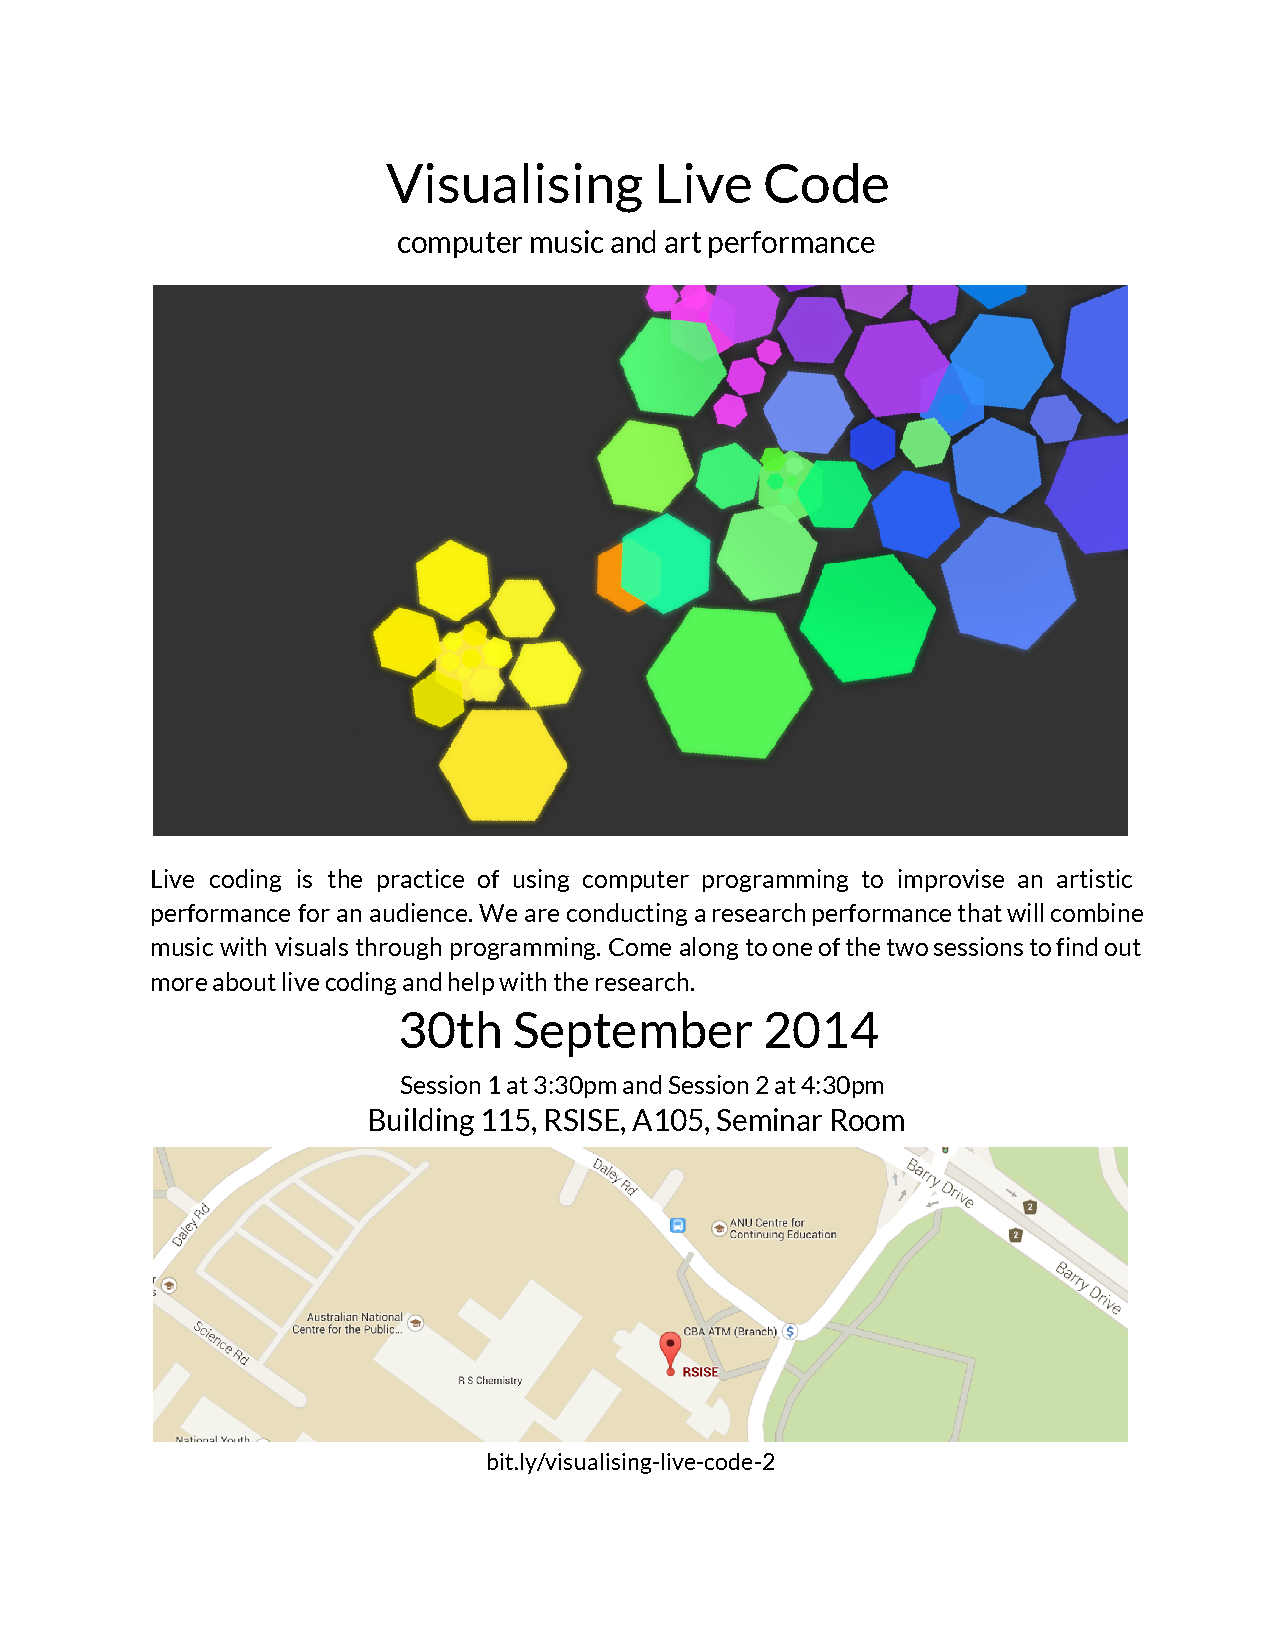
\includegraphics[page=1,width=\textwidth]{../study-3/documents/flyer-study-3.pdf}}
\end{center}


% -------------------------------------------------------------
\chapter{Follow-Up User Study Visualisations}
\label{appendix:follow-up-user-study-visualisations}


% -------------------------------------------------------------
\chapter{Follow-Up User Study Survey}
\label{appendix:follow-up-user-study-survey}

\clearpage

\begin{center}
\fbox{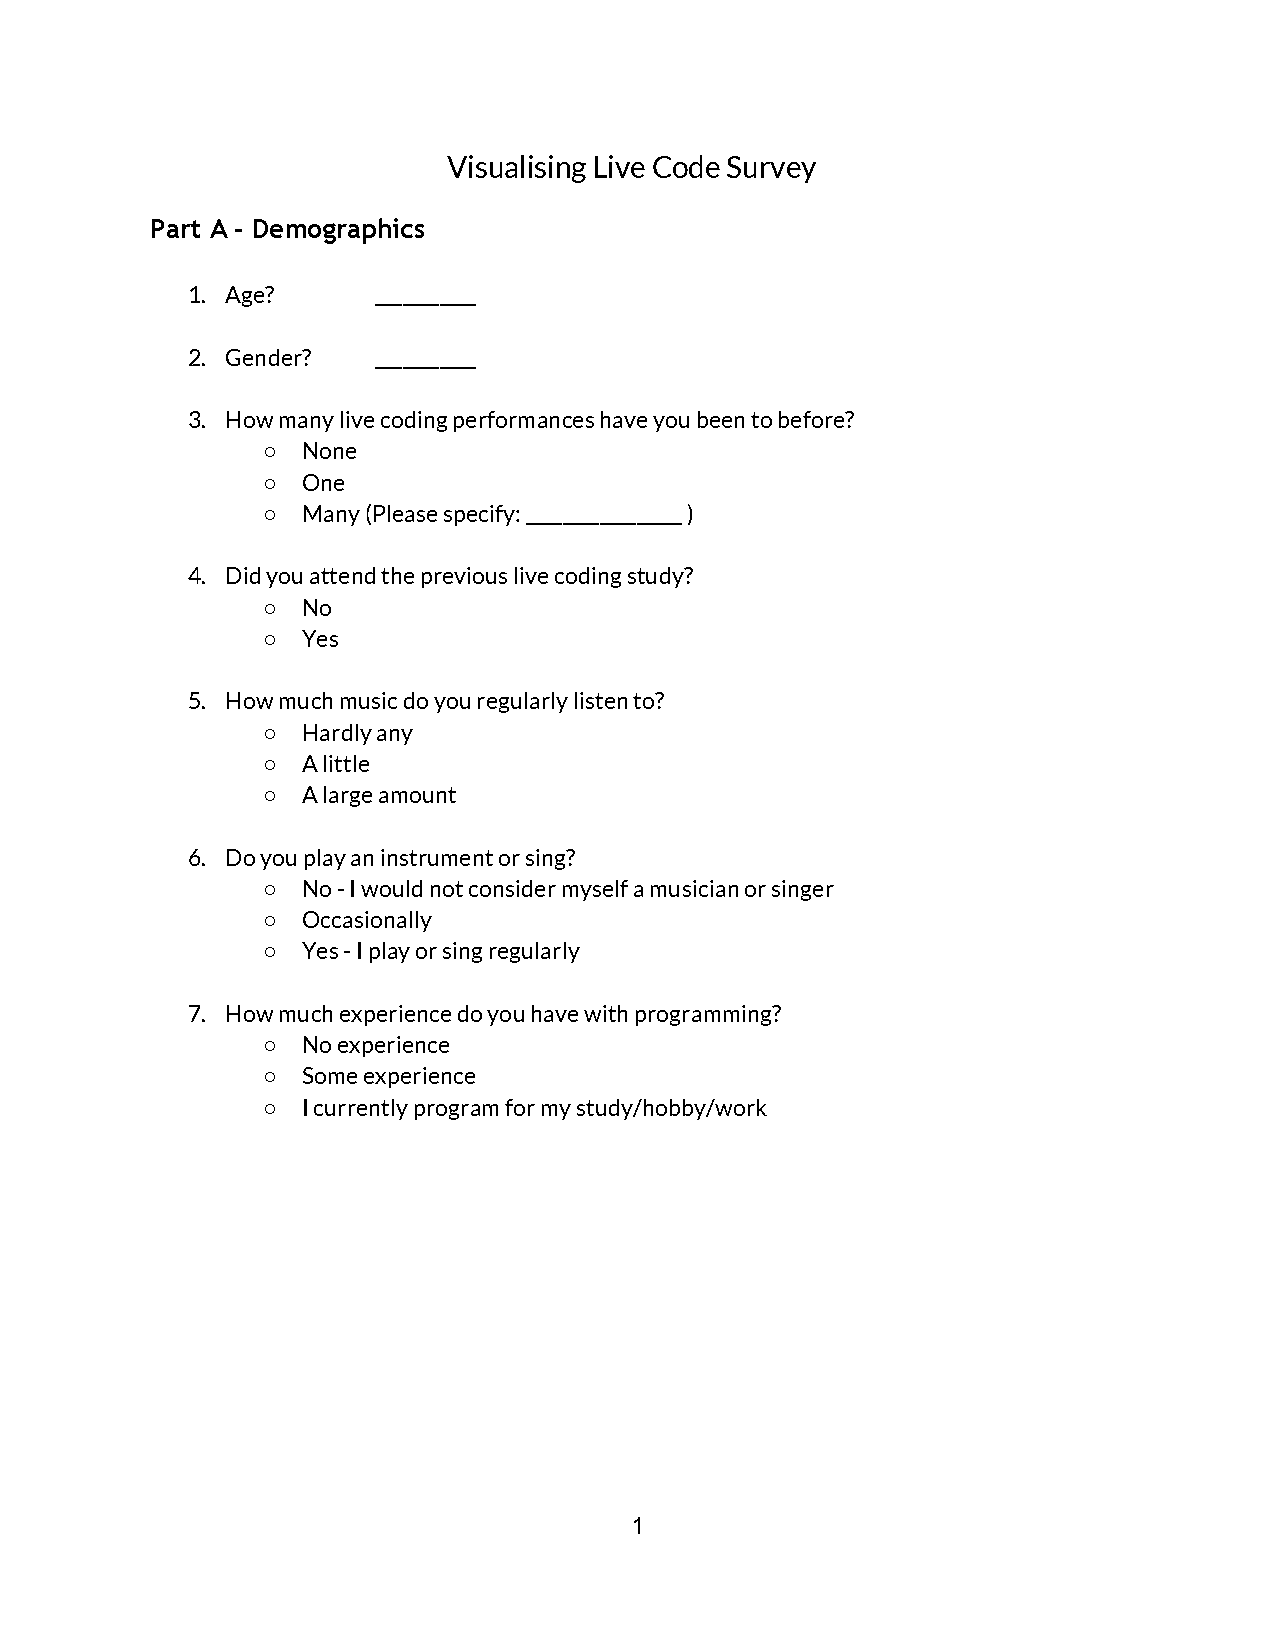
\includegraphics[page=1,width=\textwidth]{../study-3/documents/arrian-survey-study-3.pdf}}
\end{center}

\begin{center}
\fbox{\includegraphics[page=2,width=\textwidth]{../study-3/documents/arrian-survey-study-3.pdf}}
\end{center}

\begin{center}
\fbox{\includegraphics[page=3,width=\textwidth]{../study-3/documents/arrian-survey-study-3.pdf}}
\end{center}

\begin{center}
\fbox{\includegraphics[page=4,width=\textwidth]{../study-3/documents/arrian-survey-study-3.pdf}}
\end{center}


% -------------------------------------------------------------
\chapter{Follow-Up User Study Survey Results}
\label{appendix:follow-up-user-study-survey-results}


